\section{Virtual Observatory in the Electromagnetic Spectrum}
The table \ref{table:vo_EMS} shows the wavelenghts, $ \lambda $, values and
ranges for which there is a virtual observatory that contributes to design,
construction, implementation, support and/or improving of a databse with
astronomical data obtained by a specific instrument. It is sorted alphabetically
by continent and then, alphabetically by virtual observatory.\\

In the figure 2, in the first line, appears ordered the different types of
radiation with their common names. In the second line, can be located a value of
wavelenghts in meters with the type of wave, the VOs and the astronomical
instruments. A higher $ \lambda $ value is related with a lower frequency and a
lower $ \lambda $ is related with a higher frequency. The electromagnetic
spectrum value or range for each instrument (above) and virtual observatory
(below) is represented with a dot or line, respectively.\\

\begin{table*}[h!t]
\centering
\begin{tabular}{|p{1cm}|p{4cm}|p{5cm}|p{6cm}|}
    \hline                                                                      
    \textbf{VO} & \textbf{Instrument} & \textbf{Location} &
    \textbf{Spectrum value or range} \\
    \hline                                                                      
    BRAVO & Southern Astrophysical Research
    Telescope (SOAR) & Cerro Pach\'{o}n, Chile & blue (320 nm) to near infrared
    \cite{website:SOAR_EMS} \\
    \hline                                                                      
    NOVA & H-Alpha Solar Telescope for
    Argentina (HASTA) & Leoncito, San Juan, Argentina & H-Alpha (656.28 nm)
    \cite{website:HASTA_EMS} \\
    \hline
    ChiVO & Atacama Large Milimeter/submilimeter
    Array (ALMA) & Llano de Chajnantor Observatory, Atacama Desert, Chile &
    initially in 400 $ \mu $m to 3 mm \cite{website:ALMA_EMS} \\
    \hline
    \multirow{3}{3cm}{VAO} & Hubble Space
    Telescope (HST) & 569 km above the surface of Earth & near-ultraviolet,
    visible and near-infrared light with WFC3; ultraviolet light with COS;
    visible light with ACS; ultraviolet, visible and near-infrared light with
    STIS; infrared light with NICMOS \cite{website:HST_EMS} \\
     \cline{2-4}
     & Chandra X-ray Observatory & 139,000 km above the surface of Earth & X-ray
     \cite{website:Chandra_EMS} \\
     \cline{2-4}
     & Spitzer Space Telescope (SST) & 176,602,814 km above the surface of Earth
     \cite{website:SST_EMS_1} & 3 $ \mu $m to 180 $ \mu $m
     \cite{website:SST_EMS_2} \\
    \hline
    ArVO & Byurakan Astrophysical Observatory
    (BAO) & Mount Aragats, Armenia & 1.2 m and 4.2 m \cite{website:BAO_EMS} \\
    \hline
    ArVO & Spitzer Space Telescope (SST) &
    176,602,814 km above the surface of Earth & 3 $ \mu $m to 180 $ \mu $m \\
    \hline
    Vobs.it & Hubble Space Telescope (HST) & 569
    km above the surface of Earth & near-ultraviolet, visible and near-infrared
    light with WFC3; ultraviolet light with COS; visible light with ACS;
    ultraviolet, visible and near-infrared light with STIS; infrared light with
    NICMOS \\
    \hline
    \multirow{2}{3cm}{UkrVO} & Main Astronomical
    Observatory (MAO) & Kiev, Ukraine & \\
     \cline{2-4}
     & Mykolaiv Astronomical Observatory & Mykolaiv, Ukraine & \\
    \hline
    \multirow{3}{3cm}{JVO} & Subaru Telescope &
    Mauna Kea, Big Island, Hawaii & visible and infrared light
    \cite{website:Subaru_EMS} \\
     \cline{2-4}
     & Sloan Digital Sky Survey (SDSS) & Sacramento Mountains, Sunspot, New
     Mexico, USA & \\
     \cline{2-4} 
     & Atacama Large Milimeter/submilimeter Array (ALMA) & Llano de Chajnantor
     Observatory, Atacama Desert, Chile & initially in 400 $ \mu $m to 3 mm \\
    \hline
    VOI & Himalayan Chandra Telescope (HCT) & Mount
    Saraswati, Digpa-ratsa Ri, Hanle, India & infrared light 
    \cite{website:HCT_EMS} \\
    \hline
 \end{tabular}
\caption{Virtual observatories that contributes to specifics astronomical
instruments.}
\label{table:vo_EMS}
\end{table*}
%\end{longtable}
%\end{center}

\begin{landscape}
\begin{figure}%[h]
\begin{center}
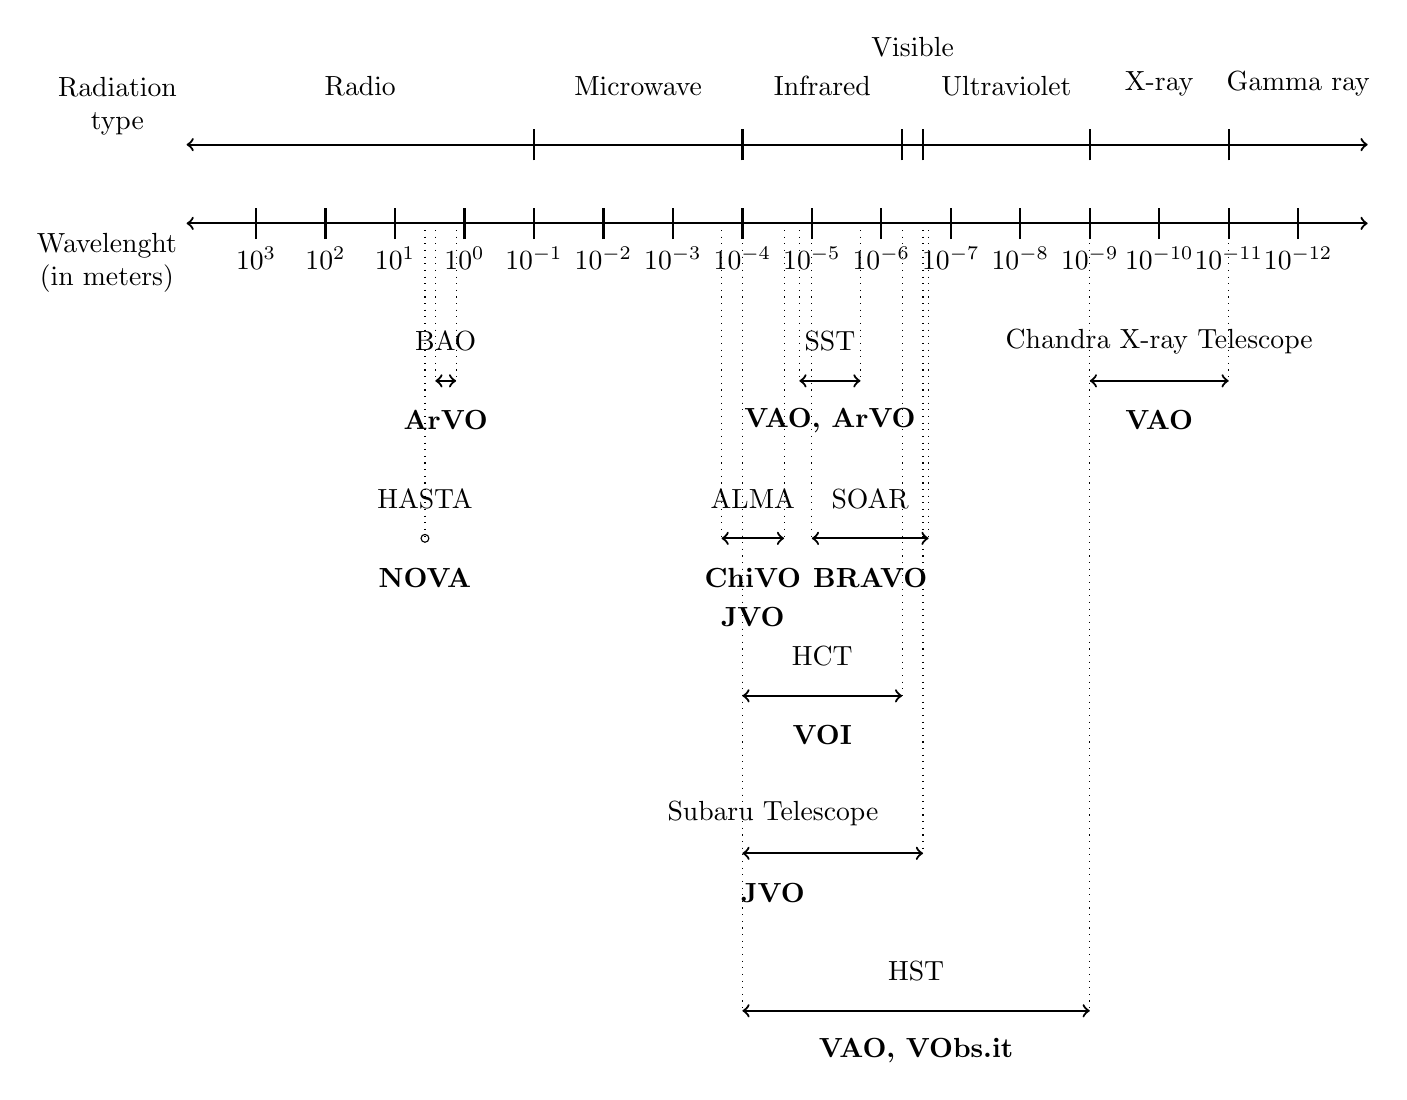
\begin{tikzpicture}
\pgfmathsetmacro{\lineLenght}{15}
\pgfmathsetmacro{\lineDivNum}{17}
\pgfmathsetmacro{\markPlace}{\lineLenght/\lineDivNum}
\def\limitsList{5,8,10.3,10.6,13,15}
\def\regionArray{{2.5,(5+8)/2,(8+10.3)/2,(10.3+10.6)/2,(10.6+13)/2,(13+15)/2,
                  (15+17)/2}}
\foreach \x in {0,1} {
  \draw[<->,thick] (0,\x) -- (\lineLenght,\x);
}
\foreach \x in \limitsList {
  \draw[thick] (\x*\markPlace,0.8) -- (\x*\markPlace,1.2);
}
\foreach \x in {1,2,...,16} {
  \pgfmathtruncatemacro{\b}{\x-2*\x+4} 
  \draw[thick] (\x*\markPlace,-0.2) -- (\x*\markPlace,0.2)
  node[pos=-0.6]{$10^{\b}$};
}
\node [anchor=north east,align=center] at (0,0) {Wavelenght\\(in meters)};
\node [anchor=south east,align=center] at (0,1) {Radiation\\type};
\node [above] at (\regionArray[0]*\markPlace,1.5) {Radio};
\node [above] at (\regionArray[1]*\markPlace,1.5) {Microwave};
\node [above] at (\regionArray[2]*\markPlace,1.5) {Infrared};
\node [above] at (\regionArray[3]*\markPlace,2) {Visible};
\node [above] at (\regionArray[4]*\markPlace,1.5) {Ultraviolet};
\node [above] at (\regionArray[5]*\markPlace,1.5) {X-ray};
\node [above] at (\regionArray[6]*\markPlace,1.5) {Gamma ray};

% Spectrum value or range for each instrument where some virtual observatory
% contributes

\pgfmathsetmacro{\factor}{\markPlace/2}
% ALMA
\draw[<->,thick] (7.7*\markPlace,-4) -- (8.6*\markPlace,-4);
\pgfmathparse{multiply(8.6-7.7,\factor)}
\node at (\pgfmathresult+7.7*\markPlace,-3.5) {ALMA};
\node at (\pgfmathresult+7.7*\markPlace,-4.5) {\textbf{ChiVO}};
\node at (\pgfmathresult+7.7*\markPlace,-5.0) {\textbf{JVO}};
 BAO
\draw[<->,thick] (3.58*\markPlace,-2) -- (3.88*\markPlace,-2);
\pgfmathparse{multiply(3.88-3.58,\factor)}
\node at (\pgfmathresult+3.58*\markPlace,-1.5) {BAO};
\node at (\pgfmathresult+3.58*\markPlace,-2.5) {\textbf{ArVO}};
% Chandra X-ray Telescope 
\draw[<->,thick] (13*\markPlace,-2) -- (15*\markPlace,-2);
\pgfmathparse{multiply(15-13,\factor)}
\node at (\pgfmathresult+13*\markPlace,-1.5) {Chandra X-ray Telescope};
\node at (\pgfmathresult+13*\markPlace,-2.5) {\textbf{VAO}};
% HASTA 
\node at (3.4312*\markPlace,-4) [inner sep=1pt,circle,draw] {};
\node at (3.4312*\markPlace,-3.5) {HASTA};
\node at (3.4312*\markPlace,-4.5) {\textbf{NOVA}};
% HCT
\draw[<->,thick] (8*\markPlace,-6) -- (10.3*\markPlace,-6);
\pgfmathparse{multiply(10.3-8,\factor)}
\node at (\pgfmathresult+8*\markPlace,-5.5) {HCT};
\node at (\pgfmathresult+8*\markPlace,-6.5) {\textbf{VOI}};
% HST  
\draw[<->,thick] (8*\markPlace,-10) -- (13*\markPlace,-10);
\pgfmathparse{multiply(13-8,\factor)}
\node at (\pgfmathresult+8*\markPlace,-9.5) {HST};
\node at (\pgfmathresult+8*\markPlace,-10.5) {\textbf{VAO, VObs.it}};
% SOAR 
\draw[<->,thick] (9*\markPlace,-4) -- (10.68*\markPlace,-4);
\pgfmathparse{multiply(10.68-9,\factor)}
\node at (\pgfmathresult+9*\markPlace,-3.5) {SOAR};
\node at (\pgfmathresult+9*\markPlace,-4.5) {\textbf{BRAVO}};
% SST
\draw[<->,thick] (8.82*\markPlace,-2) -- (9.7*\markPlace,-2);
\pgfmathparse{multiply(9.7-8.82,\factor)}
\node at (\pgfmathresult+8.82*\markPlace,-1.5) {SST};
\node at (\pgfmathresult+8.82*\markPlace,-2.5) {\textbf{VAO, ArVO}};
% Subaru Telescope
\draw[<->,thick] (8*\markPlace,-8) -- (10.6*\markPlace,-8);
\node at (\pgfmathresult+8*\markPlace,-7.5) {Subaru Telescope};
\node at (\pgfmathresult+8*\markPlace,-8.5) {\textbf{JVO}};

% Perpendicular long dotted lines

\def\firstLinesEnds{3.58,3.88,8.82,9.7,13,15}
\foreach \x in \firstLinesEnds {
  \draw[dotted] (\x*\markPlace,0) -- (\x*\markPlace,-2);
}
\def\secondLinesEnds{3.4312,7.7,8.6,9,10.68}
\foreach \x in \secondLinesEnds {
  \draw[dotted] (\x*\markPlace,0) -- (\x*\markPlace,-4);
}
\draw[dotted] (8*\markPlace,0) -- (8*\markPlace,-6);
\draw[dotted] (10.3*\markPlace,0) -- (10.3*\markPlace,-6);
\draw[dotted] (8*\markPlace,0) -- (8*\markPlace,-8);
\draw[dotted] (10.6*\markPlace,0) -- (10.6*\markPlace,-8);
\draw[dotted] (8*\markPlace,0) -- (8*\markPlace,-10);
\draw[dotted] (13*\markPlace,0) -- (13*\markPlace,-10);
\end{tikzpicture}
\caption{Virtual observatories that contributes to specifics astronomical
instruments.}
\end{center}
\end{figure}
\end{landscape}
